\documentclass[12pt,a4paper,twoside]{report}
\usepackage[T1]{fontenc} 
\usepackage[french]{babel}
\usepackage[ansinew,utf8]{inputenc}

\usepackage{graphicx}
\usepackage{color}
\usepackage{rotating}
%\usepackage[top=2.5cm,bottom=2cm,left=2.5cm,right=2cm]{geometry}
\usepackage[left=1.1in,right=0.95in,top=1in,bottom=1in]{geometry}
\usepackage{caption}
\linespread{1.1}
\usepackage{setspace}
\usepackage{microtype}
\usepackage{gensymb}
\usepackage[toc,page]{appendix}
\usepackage{textcomp}
\usepackage{makeidx}
\usepackage{multirow}
\usepackage[french]{minitoc}
\setcounter{minitocdepth}{1}
\usepackage{eurosym}
\definecolor{gray}{rgb}{.7,.7,.7}
\definecolor{Prune}{RGB}{99,0,60}
\usepackage[dvipsnames]{xcolor}
\usepackage{mdframed}
\usepackage{lmodern}
\usepackage{subfig}
\usepackage[Lenny]{fncychap}
\usepackage{calc}
\usepackage{float}
\usepackage{booktabs}
\usepackage{epstopdf}
\usepackage{pgf,tikz}
\usepackage{schemabloc}
\usepackage{caption}
\usetikzlibrary{circuits}
\usepackage{amsmath,amssymb,amsfonts,amsbsy}
\usepackage{dsfont,pifont} 
\usepackage{nopageno}
\usepackage{mdframed}
\usepackage{multirow} %% Pour mettre un texte sur plusieurs rangées
\usepackage{multicol} %% Pour mettre un texte sur plusieurs colonnes
%\usepackage{scrextend} %Forcer la 4eme  de couverture en page pair
\usepackage{textpos}
\usepackage{pdfpages}

\makeindex
\begin{document}

\dominitoc

\begin{center}
{\Huge{Institut Supérieur d'Electronique de Paris}} \\
\vspace{0.5cm}

\includegraphics[scale=0.4]{ISEP.png} \\
\vspace{0.7cm}
{\Large{Cycle International Intégré (CII)}} \\
\vspace{0.7cm}
{\Large{CT.1104 : BE Robotique}} \\
\vspace{0.7cm}
{\Huge{\textbf{Robot NAO assistant dans}}} \\
\vspace{0.35cm}
{\Huge{\textbf{un magasin}}} \\
\vspace{0.3cm}
\begin{table}[h]
\begin{tabular}{cll}
\textbf{Groupe ... :} &  &  \\
\vspace{0.2cm}
 & NOM Prénom, & NOM Prénom \\
\vspace{0.2cm}
 & NOM Prénom, & NOM Prénom \\
 & NOM Prénom, & NOM Prénom \\
\end{tabular}
\end{table}
\vspace{0.2cm}
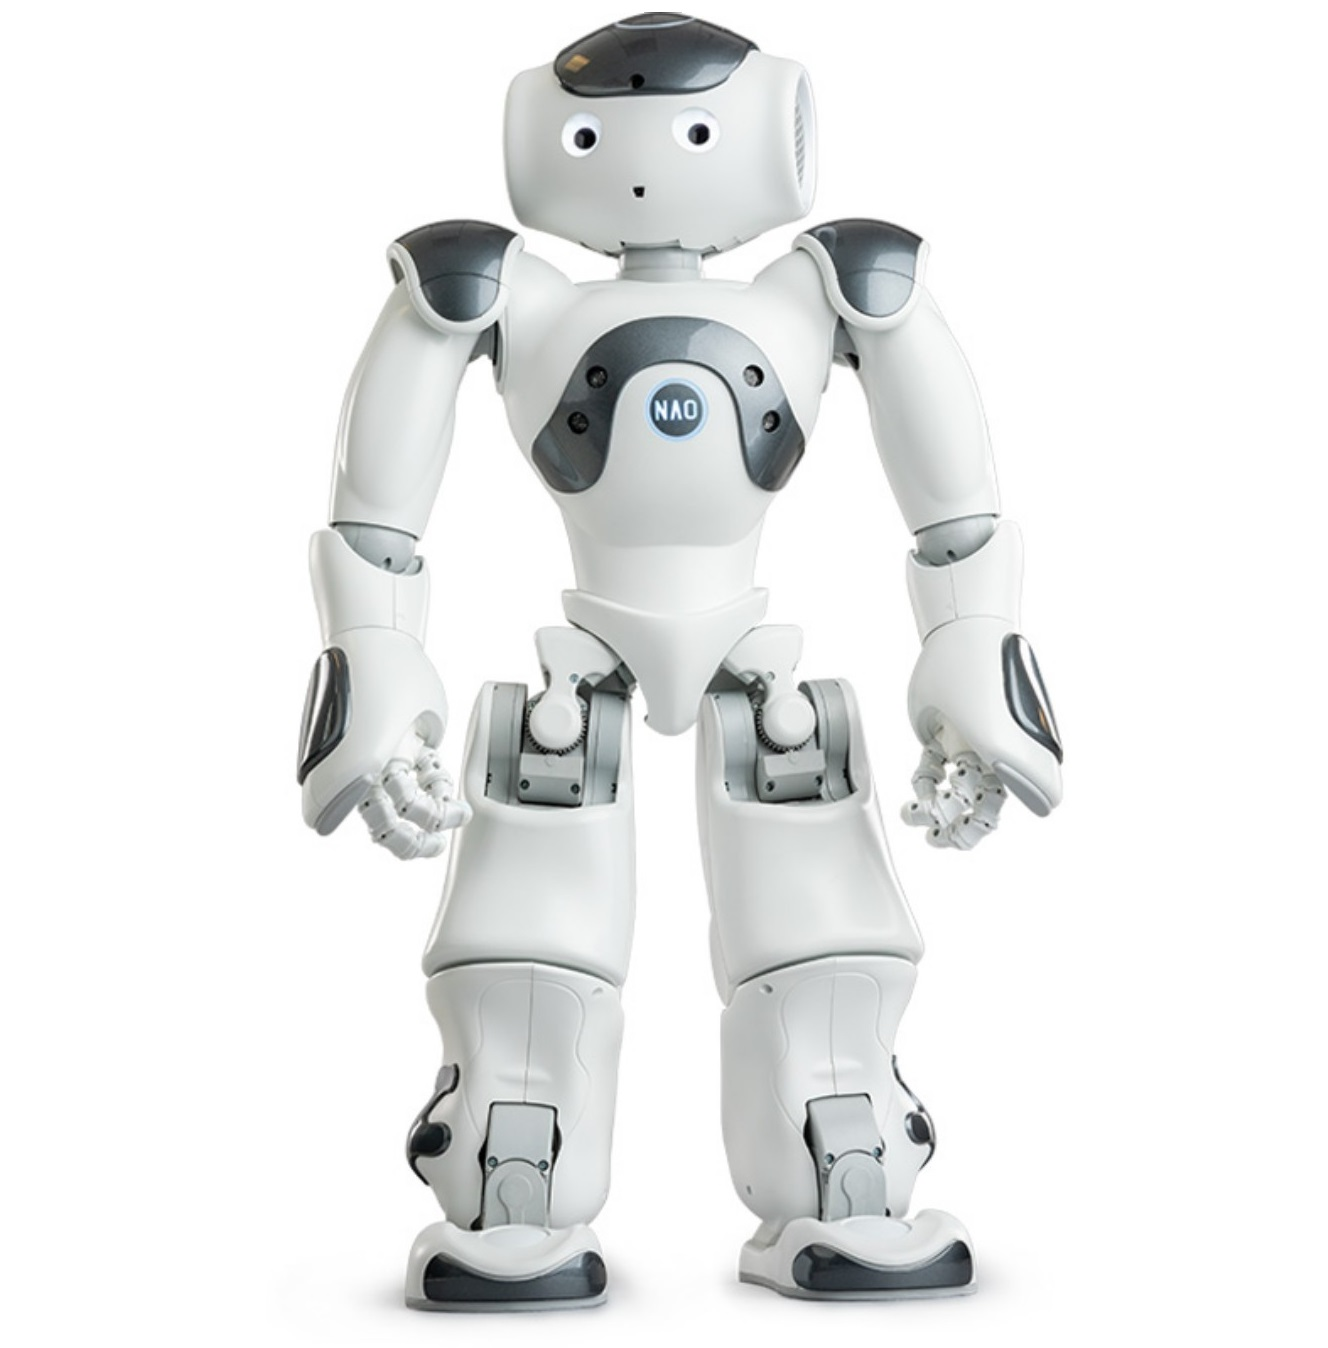
\includegraphics[scale=0.32]{NAO.jpg} \\
\vspace{0.3cm}
2021/2022
\end{center}
\vspace{-2cm}

\end{document}

